\chapter{La cryptographie à travers l'histoire}
Avant de commencer à décrire la cryptographie en soit, voyons un peu
son histoire, son apparition, et son évolution au fil du temps.

\section{L'apparition de la cryptographie}
La cryptographie serait apparue pour la première fois il y a 4000 ans,
au bord du Nil, où un scribe aurait tracé d'une façon spéciale des
hiérogliphes sur la tombe de son maître, bien que ce n'était pas
vraiment dans le but de rendre le texte illisible, mais de le rendre
plus solennel. \\

La seconde trace de cryptographie date du \bc{XVI}, c'est une tablette
d'argile sur laquelle un potier aurait écrit sa recette en enlevant
les consonnes et en changeant l'orthographe de certains mots. \\

À cette époque là, les seuls moyens utilisés pour cacher les messages
ressemblaient plus à de la stéganographie qu'à de la cryptographie,
les messages ne sont pas rendus illisibles, mais sont cachés. Par
exemple, aux de -600, Nabuchodonosor rasait le crâne d'un esclave,
écrivait un message dessus, et une fois que les cheveux avaient
repoussés, l'esclave allait chez le destinataire du message, qui lui
rasait les cheveux pour le lire. Un autre exemple est celui d'Harpage,
qui était chargé de tuer Cyrus, le petit fils du roi de Mèdes, mais
qui ne le fait pas. Par la suite, quand Cyrus aura grandit, pour
communiquer avec lui, Harpage cache les lettres dans le ventre de
lièvres, qu'il recouds par la suite. De cette façon, le message passe
inaperçu. \\

Les premières « vraies » techniques de cryptographie apparaissent
quant à elles à partir du \bc{VI}, avec une méthode de substitution,
nommée \emph{atbash}, qui consiste à remplacer les lettres par la
lettre « opposée », c'est-à-dire que A sera remplacé par Z, B par Y,
et ainsi de suite. \\

\begin{figure}[h]
  \begin{center}
    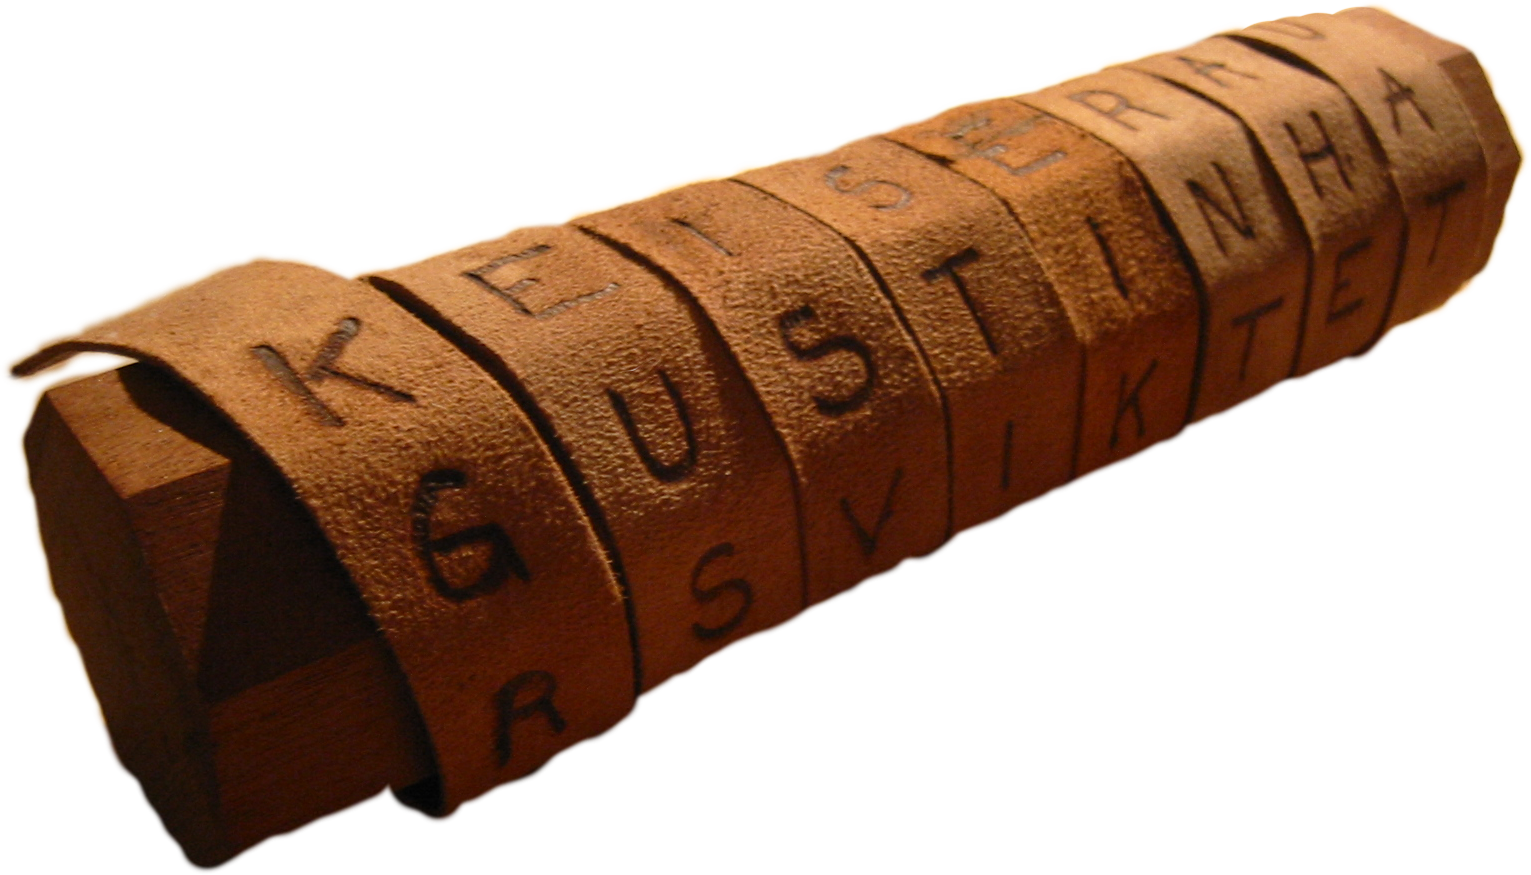
\includegraphics[scale=0.15]{eps/scytale}
  \end{center}
  \caption{La scytale des spartiates (\bc{V})}
  \label{fig:Scytale}
\end{figure}
  
Ensuite, au \bc{V}, les spartiates utilisaient pour communiquer le
bâton de Plutarque, plus connu sous le nom de \emph{scytale}. Cette
technique consistait à enrouler un long et étroit morceau de parchemin
autour d'un bâton, on écrivait ensuite le message sur le parchemin, et
on envoyait ce parchemin déroulé au destinataire, qui possédait un
bâton
de même diamètre pour déchiffrer le message. \\

Le premier réel système cryptographique par substitution est inventé
par un historien grec, Polybe aux alentours de 150 avant J.-C. (nous
verrons ce système en détail dans le chapitre \ref{syst:CarrePolybe} (page
\pageref{syst:CarreColybe}). \\

\label{syst:ChiffreCesar}
Pendant le \bc{I}, les armées de César utilisaient une méthode de
chiffrement par substitution simple, qui consistait à décaler les
lettres de l'alphabet d'un certain rang dans l'alphabet (de 3 rangs la
plupart du temps, ainsi A devient D, B devient E, \dots). Cette simple
méthode est une des méthodes de chiffrement les plus connues et à été
utilisées de nombreuses fois par la suite dans des formes dérivées (chiffre de
Vigenère\footref{syst:ChiffreVigenere}, rot13\footref{syst:rot13}), ou même
de la même façon (pendant la guerre de sécession par exemple)

\begin{figure}[h]
  \begin{center}
    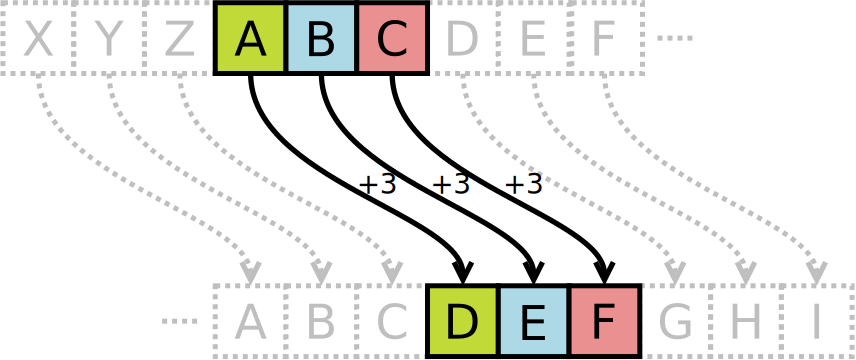
\includegraphics[scale=0.4]{eps/chiffrecesar}
  \end{center}
  \caption{Le chiffre de César}
  \label{fig:chiffrecesar}
\end{figure}

Au Moyen-âge, comme la plupart des sciences, la cryptologie n'évolue
presque pas (une personne pratiquant la cryptologie peut être
considéré comme faisant de la magie noire), à part quelques exceptions
au Moyen-Orient et en Asie (dans le Kama-sutra, il est dit que les
femmes doivent apprendre le \emph{mlecchita-vikalpa} (l'art de
l'écriture secrète) pour cacher leurs liaisons.). Il faut donc
attendre le XV\ieme~ siècle pour que la cryptographie commence
réellement à évoluer. \\

\section{L'évolution de la cryptographie}
Au début du XV\ieme~ siècle donc, un égyptien écrit une encyclopédie en
24 volumes comprenant une partie sur la cryptologie qui décrit des
chiffres de substitution et de transposition. Le premier chiffre de
substitution polyalphabétique\footref{SubstitutionPolyalphabetique}
est inventé par Leone Battista Alberti en 1467, un humaniste italien
de la reinaissance, aussi connu pour ses travaux en architecture,
surnommé \emph{Le père de la cryptographie occidentale} par
l'historien David Kahn\cite{Codebreakers}. Cette technique est appelée
le \emph{cadran chiffran}\label{syst:cadranchiffran}, ce sont deux
disques de 24 cases attachés, contenant les lettres de l'alphabet (le
premier en contient 20, H, K et Y n'étant pas « indispensables », J, U
et W n'étant pas dans l'alphabet latin, les 4 autres cases sont
occupées par des chiffres. L'autre disque contient les 23 lettres
latines dans un ordre aléatoire et le signe \&). Le plus petit disque
peut tourner, les lettres claires et chiffrées se trouvent alors face
à face, et il suffit de recopier la lettre du petit disque pour
chiffrer la lettre du grand disque. Après avoir chiffré quelques
lettres, on décale le disque et on continue ainsi de suite, en
indiquant sur le message chiffré le changement. Dans son ouvrage, il
parle aussi de cryptanalyse, et il introduit le concept d'analyse des 
fréquences. \\

\begin{figure}[h]
  \begin{center}
    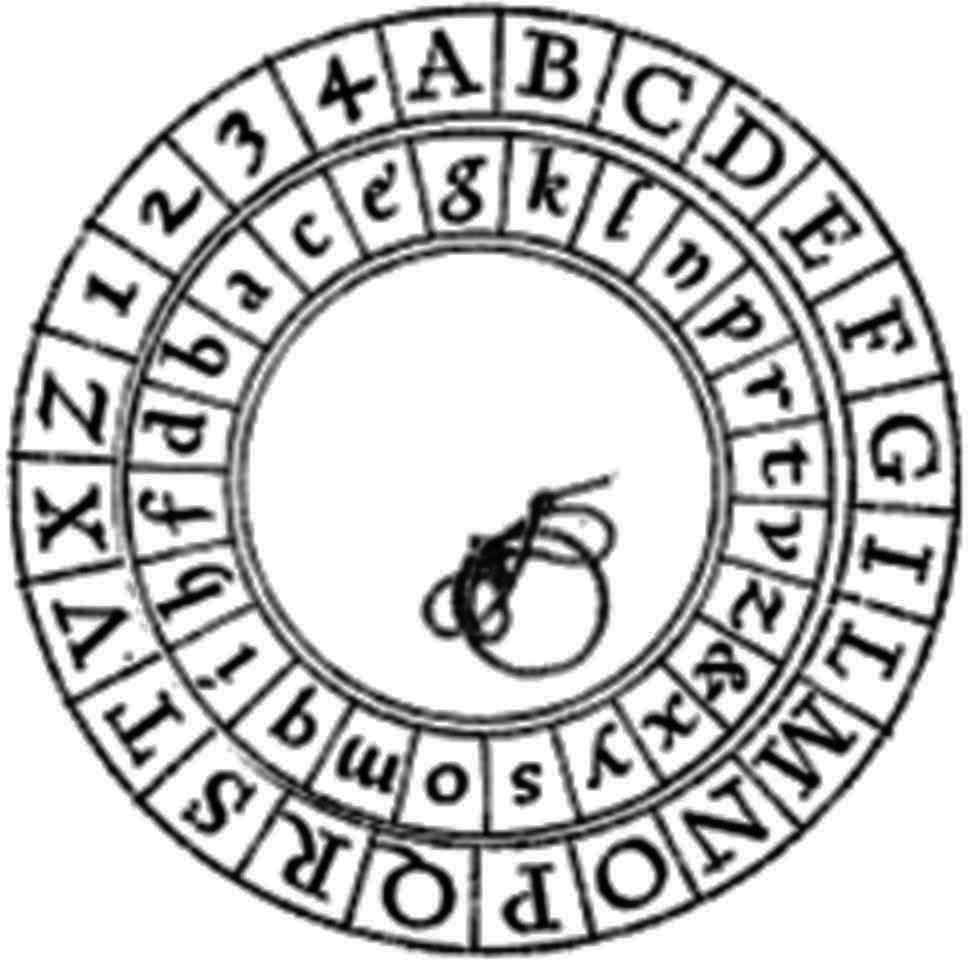
\includegraphics[scale=0.2]{eps/AlbertiCipherDisk}
    \hspace{3cm}
    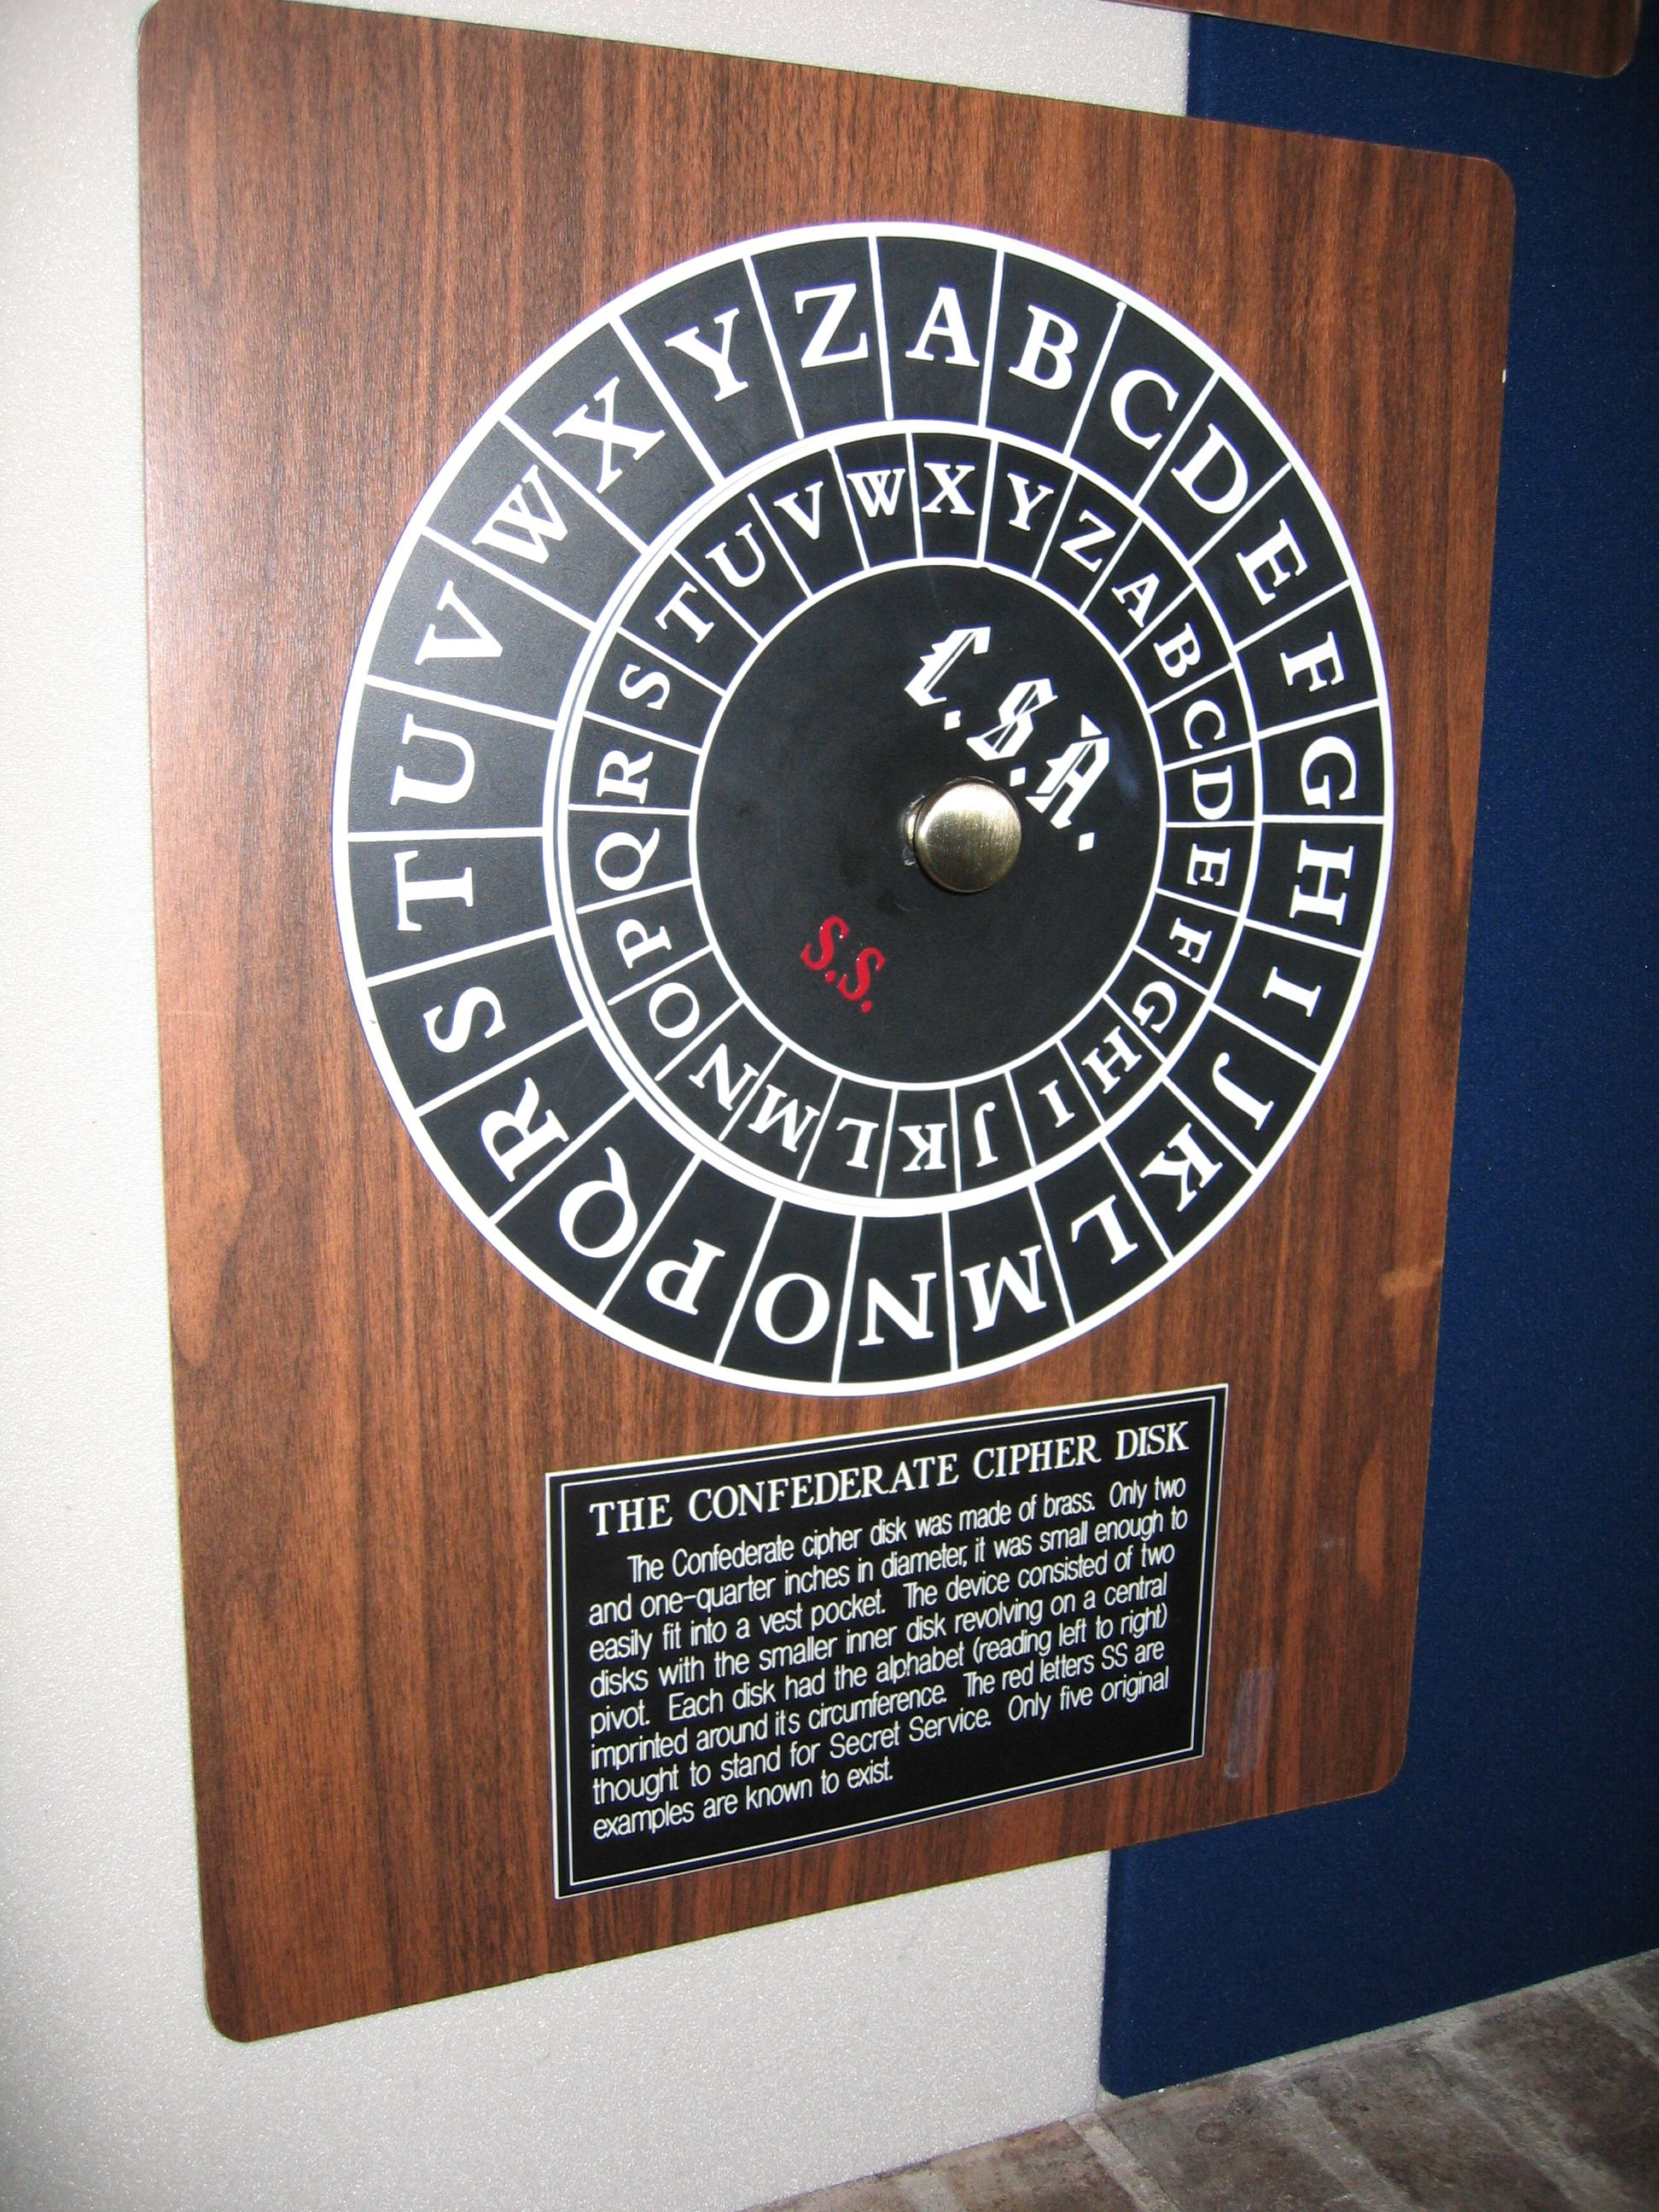
\includegraphics[scale=0.15]{eps/ConfederateCipherDisk}
  \end{center}
  \caption{Le cadran chiffrant d'Alberti, dans sa forme originelle à
    gauche, et réutilisé par les confédérés pendant la guerre de
    sécession}
  \label{fig:AlbertiCadranChiffrant}
\end{figure}

En 1518, Jean Trithème publie Polygraphi\ae , le premier livre imprimé
sur la cryptologie, où il invente un chiffre stéganographique, et ce
qui deviendra par la suite le chiffre de
Vigenère\footref{syst:Chiffrevigenere}. \\

Au milieu du XVI\ieme~ siècle, Jérôme cardan invente le premier
\emph{procédé autoclave} (qui utilise le message clair comme clef),
mais ce système comporte des lacunes. Il invente aussi la \emph{grille
  de Cardan}, un système stéganographique qui cache un message dans
une grille de lettres. Pour lire le message, il faut utiliser un cache
troué d'une certaines façons, les lettres apparaissent alors dans les
trous, et on peut lire le message. \\

\begin{figure}[h]
  \begin{center}
    \includegraphics[scale=0.2]{eps/GrilleCardan}
  \end{center}
  \caption{Un exemple de grille de Cardan}
  \label{fig:GrilleCardan}
\end{figure}

% Premières techniques de cryptographie
% Plus vieux document chiffré : un potier qui écrit sa recettes en
% enlevant des consonnes et en changeant l'orthographe des mots.
% En chine : stégano (papirus enroulé en boule recouvert de cire, avalé)
% première trace : vers 2000 av J.-C.
% Scytale -500 av J.-C. : == bâton de Plutarque.
% Spartiates, bâton rond, qu'on entoure d'un long et étroit morceau de
% parchemin. Une fois mis autour, on écrit le message dessus, puis on
% l'envoie au destinataire, qui possède une scytale de même diamètre,
% et qui déchiffre donc facilement le message. Fa
% Nabuchodonosor : -600 av J.-C. : 
% On rase le crâne d'un esclave, et une fois les cheveux repoussés, on
% l'envoie au destinataire, qui rase à nouveau les cheveux.
% Harpage qui envoie un message à Cyrus, il ouvre le ventre d'un
% lièvre pour y cacher une lettre, et l'envoya à Cyrus.
% Hebreux : Vieme av JC, atbash, chaque lettre est inversée A->Z,
% B->Y, ...

% ~-200 : premiers "vrais" systèmes cryptographiques : 
% caré de polybe, historiengrec : ~-150
% 1er siècle avant J.-C. : 
% code de césar utilisé dans l'armée romaine, réutilisé par la suite
% durant la guerre de sécession et l'armée russe en 1915 (rot13)

% Moyen age : quasi rien car sorcellerie, tout ça.

% Quasi rien jusqu'au XVieme 
%XV : encyclopédie de 14 volume écrite par un égyptien Abd Allah
%al-Qalashandi qui inclut une section sur la cryptologie. Elle y
%décrit des chiffres de substitution et de transposition.
% Leon Battista Alberti, humaniste italien de la renaissance,
% architecte, écrivain, philosophe et peintre. IMAGE
% écrit un essai parlant de cryptanalyse, avec
% l'analyse de fréquences des lettres en latin et italien. Invente
% aussi le cadran chiffrant, première méthode de chiffrement
% polyalphabétique.
% Cadran chiffrant : 2 disques contenant les lettres de l'alphabet, 
%dont un qui tourne (20 lettres chez Alberti, et le cadran faisait 24
%cases, JUW pas dans l'alphabet, et on omet H et K et Y (« qui ne sont pas
%indispensables », le deuxième cadran contient les 23 lettres latines
%+ le &) Après avoir chiffré 3 ou 4 lettres, on décale le disque, et
%on l'indique en notant de le message la lettre au dessus du k(lettre
%sur le petit).
% Notion de surchiffrement aussi. (à relire)

% 1518 : Jean trithème écrit Polygraphiae, premier livre imprimé sur
% la cryptologie, où il invente un chiffre stéganographique et ce qui
% deviendra par la suite le chiffre de Vigenère. voir la bonne partie

% Pendant certaines guerres en europe, les espagnols communiquaient
% via un chiffre, qu'ils changaient de temps en temps afin de troubler
% les gens qui pourraient essayer de le déchiffrer. Certaines lettres
% furent interceptés, et Henri IV chargea un géomètre, Viete, de
% trouver la clé de ces lettres. Il y réussit brillement, en
% comprenant le chiffre dans toutes ses formes possibles. La Cour
% d'Espagne, accusa le gouvernement français d'avoir recouru à des
% serciers, et voulait que Viete soit jugé comme un négromant en
% portant des plaintes à Rome. Il n'en fut rien mais à cette époque
% encore, c'était très dangereux d'être considéré comme un sorcier.

% Milieu du 16ème, Jérôme cardan invente le premier procédé autoclave,
% et une méthode stéganographique connue sous le nom de grille de
% cardan, où il cache le message dans une "grille de lettres", on
% retrouvera le message facilement 


En 1553, Giovan Batista Belaso utilise le terme \emph{clé
  litérale} ou \emph{mot de passe} pour des clés de petite taille
faciles à mémoriser. %TODO: plus d'infos
10 ans plus tard, Giambattista della Porta écrit une sorte
de recueil des connaissances cryptographique de cette époque. Il
invente aussi la première substitution bigrammique (voir les
substitution polygrammiques, chapitre
\ref{SubstitutionPolygrammiques}, page
\pageref{SubstitutionPolygrammiques}). Il invente aussi le premier
système de chiffrement polyalphabétique où l'on changeait d'alphabet à
chaque lettre. \\

En 1585, Blaise de Vigenère publie \emph{Traité des chiffres
  ou secrètes manières d'écrire}, où il présente une méthode
cryptographique fortement inspirée de celle de Jean Trithème. Cette
méthode sera appelée plus tard \emph{carré de Vigenère} (à tort,
elle aurait plutôt dû s'appeler carré de Trithème, Vigenère ne
l'ayant qu'un peu modifiée pour rendre l'utilisation de clé possible).
Cette méthode sera longtemps considérée comme indéchiffrable, et ne
sera que cassée au milieu du XIX\ieme~ siècle, plus ou moins
simultanément par un mathématicien anglais, Charles Babbage et
par un cryptologue russe, Friedrich Wilhelm Kasiski. \\

À la fin du XVII\ieme~ siècle, Antoine Rossignol ainsi que ses
fils par la suite travaillèrent pour Louis XIV. Avec son fils,
Bonaventure, il élabore le \emph{Grand Chiffre}, un système de
chiffrement par substitution à répertoire, qui était considéré comme
incassable, et est rendu indéchiffrable après le décès de ses auteurs,
qui emportèrent sont secret. Ce chiffre sera néanmoins cassé 1893 par
Étienne Bazeries. Il s'avère qu'il introduisait entre autre
dans le message chiffré, des éléments inutiles ayant pour but de
rendre plus difficile le travail du cryptanalyste.\\

En 1793, Thomas Jefferson, futur président des États-Unis,
invente une méthode de substitution polyalphabétique (nommée le
\emph{cylindre de Jefferson}) qui consiste en
un cylindre formé de 26 roues, où est écrit l'alphabet dans un ordre
aléatoire et différement sur chacune des roues. On peut placer les
roues dans l'ordre qu'on veut (l'ordre correspondant à la clé).
Une fois les roues placées suivant la clé, on les déplace de façon à
former le message sur une ligne. Il ne reste plus qu'à recopier une
autre ligne pour avoir le message chiffré. Le récepteur du message
chiffré le formera alors sur son cylindre, dont les roues aurant au
préalables été placées selon la clé, et il lui restera à trouver la
ligne contenant le message (la seule ligne intelligible). Ce procédé
fut réinventé par le colonel français Brazeries, et réutilisé
dans l'armée américaine entre 1923 et 1942 (sous le nom de M-94, la
machine est un peu modifié).

\begin{figure}[h]
  \begin{center}
    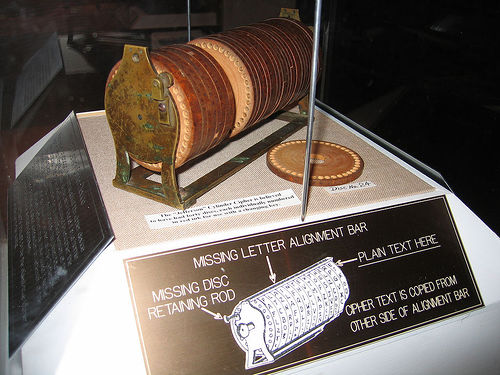
\includegraphics[scale=0.4]{eps/jeffersonDisk}
    \hfill
    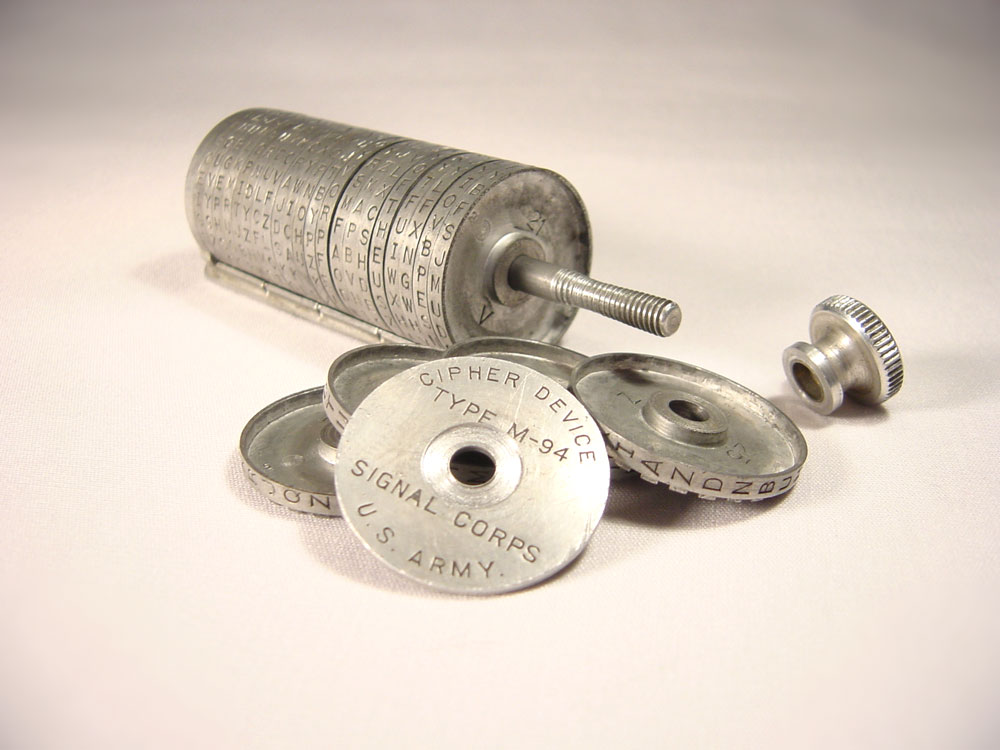
\includegraphics[scale=0.25]{eps/m94}
  \end{center}
  \caption{À gauche, un disque de Jefferson du XVIII\ieme~ au musée
    national de cryptologie de la NSA, 
    à droite, un exemplaire du M-94}
  \label{fig:JeffersonDisk}
\end{figure}

Fin XIX\ieme, Charles Wheatstone invente un chiffre
polygrammique que nous verrons en détails plus tard, ce chiffre
portera le nom de la personne l'ayant popularisé : le chiffre
  de Playfair. \\

Ensuite, viennent plusieurs avancées cryptanalytiques avec, comme nous
l'avons vu plus haut, Charles Babbage qui casse le chiffre de
Vigenère, mais ne publie pas sa découverte. Friedrich Kasiski
le casse aussi (sans avoir connaissance des travaux de
Babbage) en 1861, et publie ses travaux. En 1891, Étienne
  Bazeries casse quant à lui le Grand chiffre de Louis XIV. 

En 1883, Auguste Kerckhoffs publie deux articles sur la
cryptographie militaire, où il explique des règles qui peuvent être
considérées comme les règles de base d'un système cryptographique
sûr. Nous verrons ces règles en détail dans le chapitre
\ref{PrincipeKerckhoffs}. \\

\section{La cryptographie pendant la Première Guerre mondiale}
La cryptographie était très présente pendant les guerres, d'où
l'importance des cryptanalystes. Pour cela, chaque état avait recours
à ses cryptanalystes pour décoder les messages ennemis interceptés (ou
même alliés, c'était le cas de l'Angleterre qui écoutait les
communications entrantes et sortantes aux États-Unis).

L'organisme de déchiffrement sûrement le plus important lors de cette guerre
est connu sous le nom de \emph{Room 40} (Bureau 40), le service de
déchiffrement britannique de la \emph{Royal Navy}, qui aurait déchiffré
plus ou moins 15.000 communications allemandes, la plus grosse affaire
connue étant celle du télégramme de Zimmerman.

Zimmerman était le ministre allemand des affaires étrangères durant la
guerre. En janvier 1917, alors que les États-Unis sont neutres,
Zimmerman envoie un message codé à l'ambassadeur du Mexique aux
États-Unis, qui devrait être retransmit au président Mexicain après
avoir été déchiffré, message qui est intercepté par les services
secrets britanniques, qui charge immédiatement le Bureau 40 du
déchiffrement du message. Un mois plus tard, c'est chose faite ; le
message indiquait que les allemands souhaitaient déclencher une guerre
sous-marine totale, et qu'il serait difficile que les États-Unis
restent neutres. L'empire Allemand propose alors une alliance avec le
Mexique, avec une aide financière pour reconquérir le Texas, le
Nouveau-Mexique et l'Arizona. Il était aussi demandé d'essayer de
convaincre les Japonais d'entrer en guerre contre les États-Unis.
Le message est finalement transmit aux gouvernement américain après
quelques démarches évitant aux anglais de devoir dire aux américains
qu'ils écoutaient leurs communications diplomatiques, et le télégramme
fut publié dans la presse américaine le $1^{er}$ mars. Le 6 avril, les
États-Unis rentrent en guerre contre l'Allemagne, le Congrès ayant
accepté la demande du président Wilson. Bien que le télégramme n'est
pas la seule cause de l'entrée en guerre des États-Unis, il fit
fortement évoluer l'opinion publique américaine dans un sentiment
anti-allemand.

Le Bureau 40 fusionnera après la guerre avec le MI1 (département des
services secrets britannique chargé du décryptage) pour former le
\emph{Government Code and Cypher School}, qui sera encore utile
pendant la Seconde Guerre mondiale, sous le nom de \emph{Government
  Communications Headquarters} \\

\begin{figure}[h]
  \begin{center}
    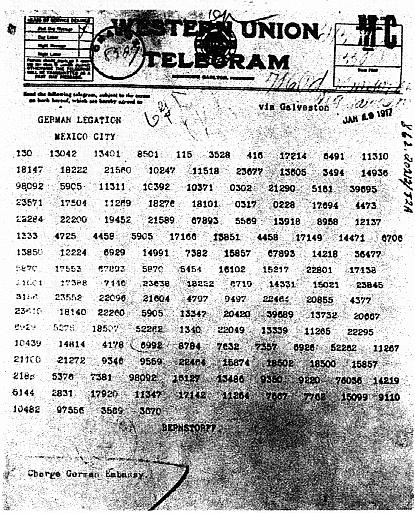
\includegraphics[scale=0.4]{eps/ZimmermanTelegram}
  \end{center}
  \caption{Photo du télégramme original envoyé par Zimmerman}
  \label{fig:JeffersonDisk}
\end{figure}

En 1917, Gilbert Vernam invente le \emph{masque jetable}, le
seul procédé cryptographique connu comme étant impossible à casser. Ce
procédé n'est pas directement utilisé car il pose des difficultées de
mise en place (problèmes de génération et de transmission des clés,
qui doivent être uniques) %TODO: voir en détail ?

%TODO: Room 40 (codebreakers, p 127 -> 150)
% Room 40 : nom du service de déchiffrement de la Royal Navy
% britannique des codes ennemis
%  déchiffré ± 15000 message
% rôle important : savoir les mouvements de la flotte allemande
% Plus grosse affaire : télégramme Zimmerman
% Fusionne avec le MI1 en 1919, sous le nom de Government Code and
% Cypher School, qui sera utile pendant la seconde WW, sous le nom de
% Government Communications Headquarters
% (MI1 : mis en place pendant la guerre, c'est le département des
% services secrets britanniques chargé du décryptage.)
% Zimmerman
% Janvier 1917, États Unis neutres
% Un message codé envoyé par Arthur Zimmerman, ministre allemand des
% affaires étrangères à destination de l'ambassade du mexique, à
% Washington
%  est intercepté par les services secrets et le room 40 est
% chargé du déchiffrement du message. Un mois après, ils y parviennent.
% Le message destiné à l'ambassadeur du mexique aux états unis
% indiquait que les allemands souhaitaient déclencher une guerre
% sous-marine totale, mais qu'il serait difficile que les états-unis
% restent neutres. L'empire allemand propose donc une alliance avec le
% mexique, qui sera aidé financièrement pour reconquérir le Texas, le
% Nouveau Mexique et l'Arizona. Le président devait aussi essayer de
% convaincre les Japonais d'entrer en guerre contre les USA.
% Le message devait être retransmit au
% président amériquain.
% Une fois ce message décodé, tout de suite envoyé aux états unis. La
% presse répand la nouvelle est les US rentrent en guerre le 6 avril
% 1917
% Ils remarquèrent que le message utilisait une technique de
% chiffrement utilisée uniquement pour les communication diplomatique
% importantes, ils se lancèrent donc d'urgence dans le déchiffrement
% du message. Le décodage fut loin d'être simple, mais le mesage
% présentait des similitudes avec d'autres messages interceptés
% auparavant. En combinant tout cela ensembles, ils réussirent petit à
% petit à décoder le message.
%TODO:image

% Chiffre de Playfair réutilisé par les anglais
% Une version complexe du chiffre de Vigenère par les russes, cassée
% en trois jours par Hermann Pokorny
Durant la Première Guerre mondiale, de nombreux systèmes de
chiffrements utilisés étaient pour la plupart d'anciens systèmes de
chiffrements, soit réutilisés tels quels, comme le chiffre de Playfair
réutilisés par les anglais, ou bien modifiées, comme ce fut le cas
avec les russes qui utilisaient une version complexe du chiffre de
Vigenère.

Il en est de même pour le système de chiffrement ADFGX, inventé en
mars 1918 par le colonel allemand Fritz % TODO: lieutenant ? (kahn)
Nebel, qui combine une version modifiée
du carré de Polybe\footref{syst:CarrePolybe} (où les chiffres des
lignes et des colonnes sont remplacés par les lettres ADFGX) suivit d'une
transposition\footref{syst:Transposition} (on change la disposition
des colonnes du carré de Polybe). Les lettres ADFGX furent choisies de
façon à limiter le risque d'erreur de l'opérateur qui les
transmettrait en Morse (Nebel trouvait qu'elles étaient simples à
retenir quand on apprenait le Morse).

Ce système est déchiffré avec beaucoup de difficultées par le
lieutenant français Georges Painvinen avril de la même année, mais à
partir du mois de juin, les allemands compliquent le système
cryptographique en y introduisant la lettre V (ce système se nomme
alors ADFGVX). Le tableau de $5\times 5$ cases devient alors un tableau
de $6\times 6$ cases, ce qui permet l'introduction des chiffres dans
les message codés, et de rendre la cryptanalyse plus
compliquée.

Néanmoins, Painvin parvint à casser le code en moins de
deux jours. Cette cryptanalyse aurait permit d'arrêter l'offensive
des allemands de printemps 1918 et aurait été une étape décisive pour
la victoire des Alliés durant cette guerre, mais certaines personnes
ne sont pas d'accord avec cela, affirmant que lorsque Painvin proposa
sa solution au code, l'attaque des allemands avait déjà échoué. 
%TODO: image explicative ?/matrice
\section{La cryptographie pendant la Seconde Guerre mondiale}
